\documentclass[../../../Bachelorarbeit.tex]{subfiles}
\begin{document}

\subsection{Bedienkonzept}
Der letzte Abschnitt der Anlagenkozeption behandelt die Erstellung des Bedienkonzeptes. Das Bedienkonzept beschreibt die Interaktion zwischen Mensch und Maschine. Im Zentrum des Konzeptes steht die Art und Weise, wie der Bediener Befehle an die Maschine übergibt und in welcher Form er Informationen von der Maschine wieder zurück bekommt. \\ % Quelle
Das Bedienkonzept wird in dieser Arbeit in zwei Unterabschnitte unterteilt. An erster Stelle steht die Bedienung der Laboranlage über als Hardware implementierte Bedienelemente. Der zweite Unterabschnitt stellt das Bedienungskonzept über eine Softwarevisualisierung dar. Für die Nutzung des mehrachsigen Positioniersystems selbst ist die Bedienung über eine Bediensoftware von größerer Relevanz. Die Hardwareimplementierung dient lediglich als Ergänzung. Außnahme stellt die Not-Halt-Funktionalität dar, welche unabdinglich als Hardwarekomponente verbaut werden muss, um eine schnelle Reaktionszeit im Notfall/Fehlerfall zu gewährleisten (Implementation in Form von einrastenden Not-Halt-Tastern).

\subsubsection{Bedienung über Hardwarekomponenten}
Grundsätzlich erfolgt die Bedienung des Positioniersystems über ein Bedienpanel an der Front des Schaltschrankes der Anlage. Nach dem Einschalten über einen Netzschalter an der rechten Seite des Schrankes kann die restliche Bedienung über besagtes Panel vorgenommen werden.\\
Auf der linken Seite des Bedienfeldes befindet sich wie auch in \autoref{fig:my-img9} zu erkennen ist ein Vier-Wege-Richtungsgeber, über welchen später durch Tasten der einzelnen Tastelemente die beiden Achsen des Systems im Handmodus gejoggt werden können.\\
Rechts an der Schaltschrankfront ist eine Gruppierung von weiteren Tast-, Schalt und drehbaren Bedienkomponenten zu erkennen. Im linken Bereich der Gruppierung sind vier weitere Taster zu erkennen. Dabei handelt es sich um den grünen \textit{START/RESET}-Taster, den roten \textit{STOP}-Taster und zwei weiße Taster, die in dieser Arbeit als Trigger für Greifaktionen des Systems genutzt werden. Die beiden Taster können nach Belieben von Anwender umprogrammiert werden, falls ein anderer Anwendungsfall umgesetzt werden soll.\\
Weiter rechts sind zwei Potentiometer am Schaltschrank angebracht, über die separat die Geschwindigkeit der x- und z-Achse angepasst werden kann. Auf der ganz rechten Seite in \autoref{fig:my-img9} zu sehen sind oben ein Schalter für den Betriebsmodus (linke Position - Handmodus; rechte Position - Automatikmodus). Darunter ist ein Ethernetport zu erkennen, der als externe Programmierschnittstelle genutzt werden soll und intern mit einem Switsch verbunden ist, der alle Steuerungen des Systems miteinender verbindet.\\
Das letzte Bedienelement auf der Schaltschrankfront ist der \textit{NOT-HALT}-Taster (ganz unten rechts in \autoref{fig:my-img9}).

\begin{figure}[H]
    \centering
    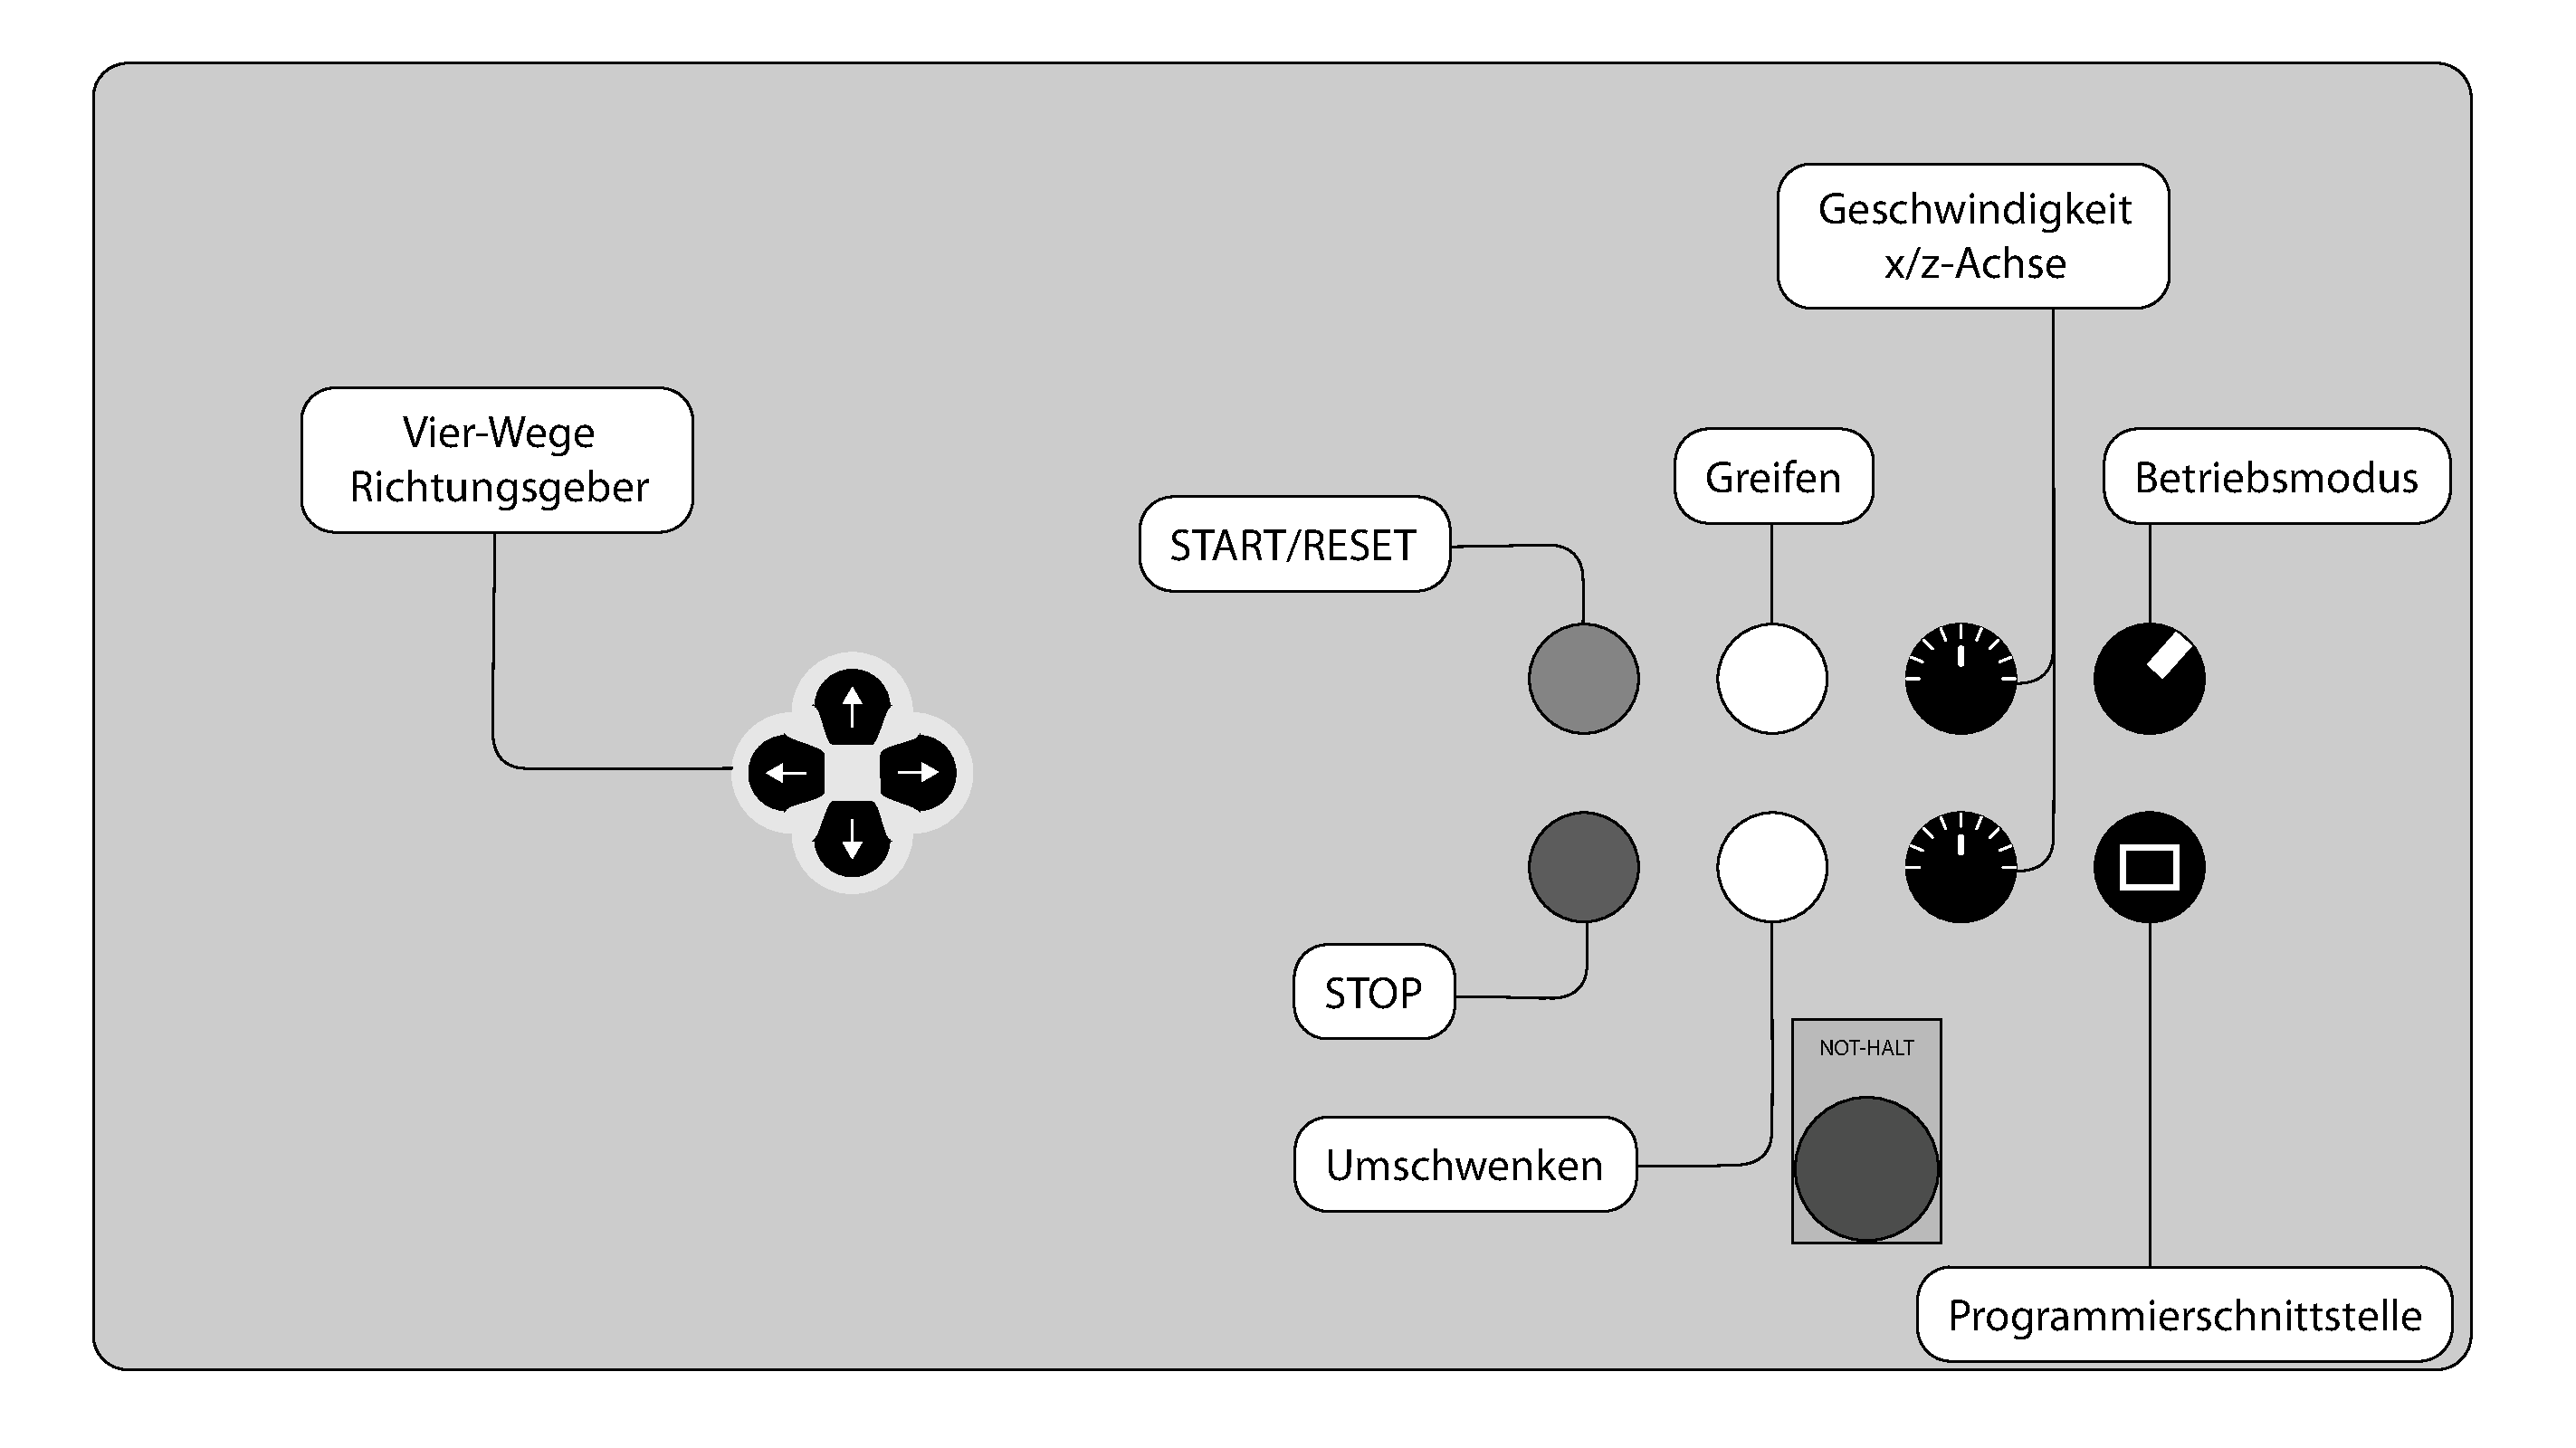
\includegraphics[width=0.7\textwidth]{Images/SchaltschrankFront.pdf}
    \caption[Bedienpanel]{Bedienpanel an der Schaltschrankfront des Positioniersystems}
    \label{fig:my-img9}
\end{figure}

Abseits der Bedienelemente am Schaltschrank finden sich noch zwei weitere Komponenten am Gehäuse der Laboranlage selbst wieder. An der äußersten linken Seite an der Front der ANlage ist ein weiterer \textit{NOT-HALT}-Taster vorgesehen. Dieser wird ergänzt duch eine zweifarbige (grün, rot) Ampel oben rechts am Gehäuse. Diese soll den aktuellen Systemzustand signalisieren (Betriebsbereit, gestoppt, in Bewegung).\\
Bereits aus dem Umfang des durch Hardwarekomponenten umgesetzten Bedienkonzeptes ist eine Notwendigkeit einer ergänzenden Softwarebedienung über eine \acs{gui} zu erkennen, um sowohl eine leichtere, als auch vollständige Bedienung nach Anforderungsvorgaben zu erfüllen.

\subsubsection{Bedienung per \acs{gui}}
Die Interaktion mit dem System soll hauptsächlich über ein mobiles Endgerät geschehen (\zB Smartphone, Tablet). Es würde sich anbieten ein \acs{hmi} \bzw ein Tablet abnehmbar an das Sysem anzubringen, um es mit diesem steuern zu können. Auf diesem soll dann eine \acs{gui} wiederzufinden sein, über welche das mehrachsige Positioniersystem bedient werden kann. \\
DAzu werden zunächst zwei Iterationen der Umsetzung geplant. Aufgrund des geringeren Entwicklungsaufwandes und somit einer Zeitersparnis könnte für grundlegende Systeminteraktionen eine reine auf Codesys 3.5 basierende Visualisierung genutzt werden. Vorgreifend zur Implementationsphase soll an dieser Stelle das \textit{MotionTemplateFull} Erwähnung findet, welches die Basis für das Steuerungsprogramm des Positioniersystems darstellen wird. Das Template besitzt bereits eine Visualisierung, die genutzt werden kann. Nachfolgende Grafik (\autoref{fig:my-img13}) zeigt die Visualisierung. Zur konkreten Bedienung der Laboranlage über die Visualissierung findet sich eine Anleitung im Kapitel Bedienungsanleitung. % Kapitelverlinkung hinzufügen !!!

\begin{figure}[H]
    \centering
    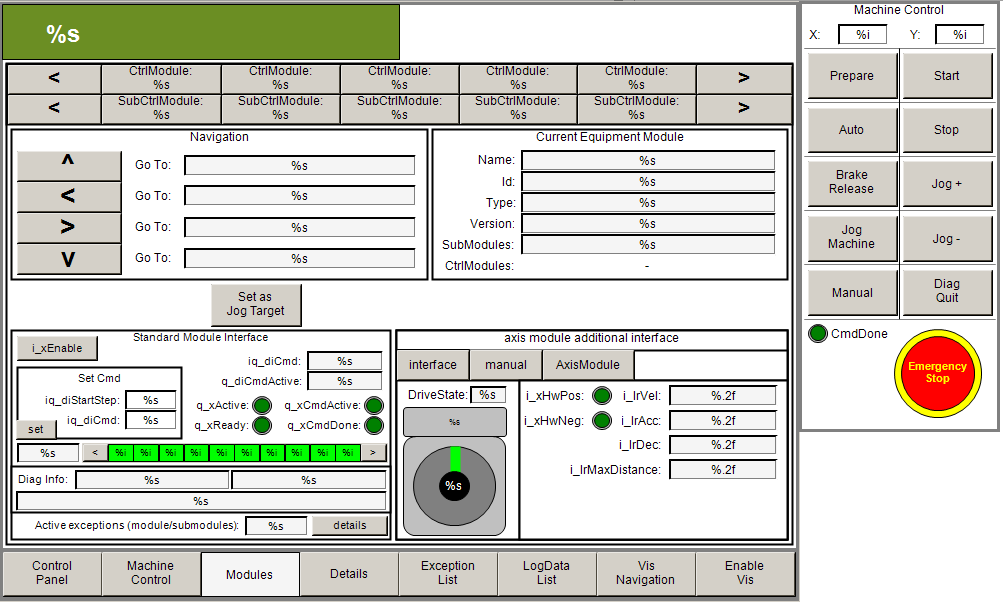
\includegraphics[width=0.7\textwidth]{Images/Visu.PNG}
    \caption[Visualisierung zur Bedienung]{Visualisierung zur Bedienung des Positioniersystems}
    \label{fig:my-img13}
\end{figure}

Wie bereits angedeutet soll die Visualisierung in \autoref{fig:my-img13} im zweiten Iterationsschritt ersetzt werden durch eine \acs{gui}. Dabei soll es sich um eine web-basierte Anwendung handeln, die über einen Backend-Service, welcher als OPC UA Client fungiert, mit dem System kommunizieren kann. Der Service (im Folgenden als OPC Gateway bezeichnet) wird programmiert in Python 3. Dabei können zum Einen OPC Daten von der Steuerung des Systems (\acs{lmc}) entgegengenommen werden, welche zum Anderen dann über einen Webservice an eine frontend \acs{gui} weitergeleitet werden. Der Datenaustausch kann bidirektionalen erfolgen, womit die Möglichkeit besteht über die Webanwendung das System per OPC UA Datenaustausch zu steuern. \\
Ein grundlegender Entwurf ist in \autoref{fig:my-img14} dargestellt.

\begin{figure}[H]
    \centering
    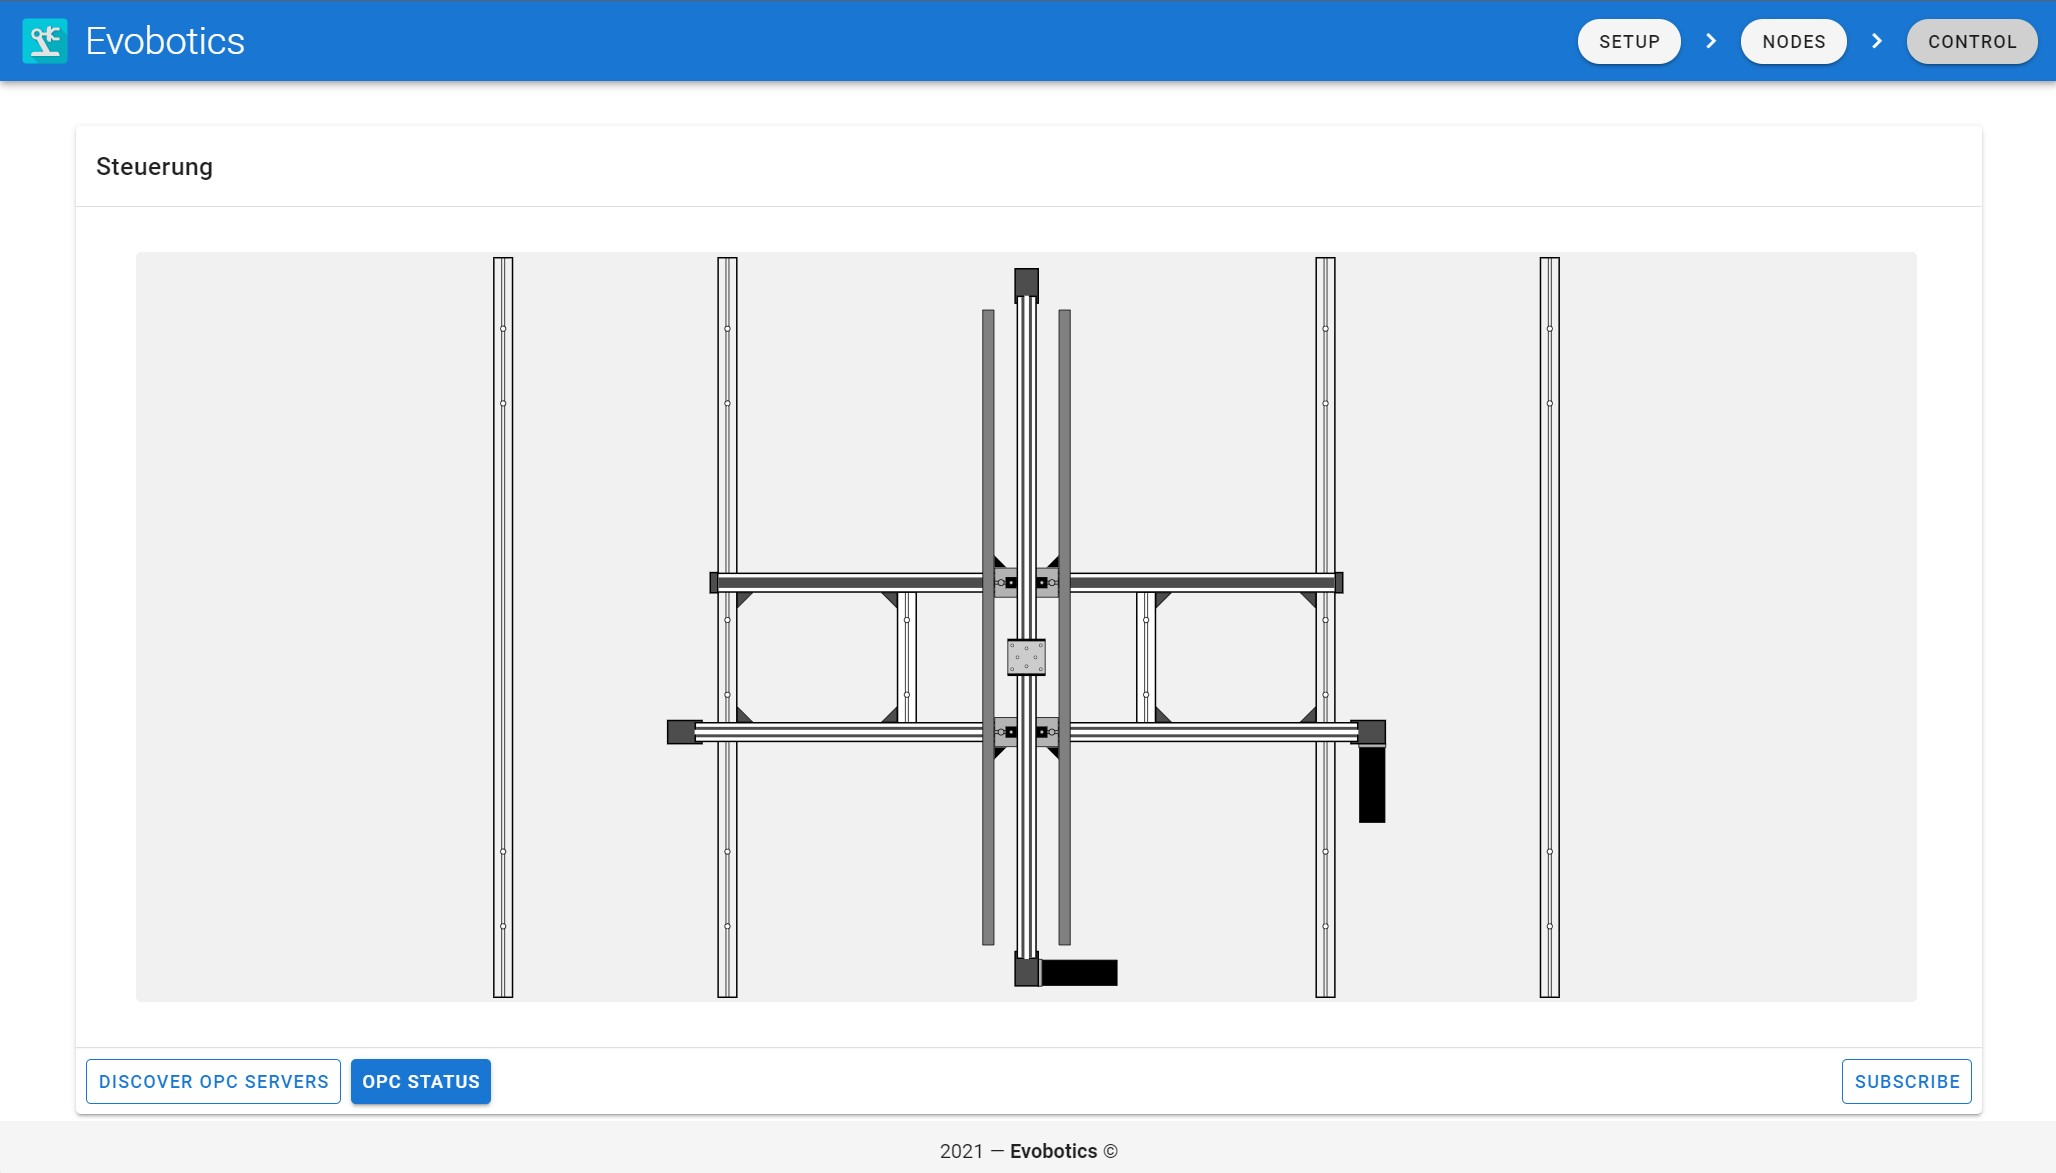
\includegraphics[width=0.7\textwidth]{Images/GUI.jpg}
    \caption[\acs{gui} zur Bedienung]{\acs{gui} zur Bedienung des mehrachsigen Positioniersystems}
    \label{fig:my-img14}
\end{figure}

Der Vorteil der web-basierten Bedienung des Systems liegt auf der einen Seite in den umfangreichen Möglichkeiten der Gestaltung, die die Visualisierungskomponenten von Codesys 3.5 um ein tausendfaches übertreffen. Auf der Anderen Seite können neue Bedienungsarten in die Oberfläche integriert werden. Die Anwendung kann nach Fertigstellung Toucheingaben entgegennehmen, um Beispielsweise absolute Positionierungsaufgaben simpel zu gestalten. Eine Erweiterung dieser Funktionalität wäre es gleich ganze Wege als TRajektorien mit dem finger \bzw einem Stift zu zeichen, die anschließend von der Positioniereinheit abgefahren werden. Die Umsetzung ermöglicht es nach Belieben Erweiterungen hinzuzufügen. \autoref{fig:my-img14} stellt somit zunächst ein grundlegendes Konzept dar und keinesfalls ein fertiges Produkt.

\end{document}